\section{Transmission Selection}

As part of your design, you will need to select the type of transmission and subsequent specification of your chosen transmission. You will need to do some research on the types of transmission to be able to present a reasoned argument for your selection. This will be followed by the steps taken to select an initial specification of transmission. In this document, we will take your through the selection of a chain transmission. For other transmission types, you will have to look up the relevant guides and processes. Do not let this put you off though as the steps are fairly similar.

\subsection{Transmission Types}

\begin{framed}
  \vspace{1cm}
    \begin{center}
      {\fontsize{50}{60}\selectfont ?}\\
      Own Research \& Lectures
    \end{center}
  \vspace{1cm}
\end{framed}

%\marginnote{Chain Drives}


% Simplex, duplex, triplex

%\marginnote{Advantages}
%\begin{itemize}
%  \item Typically stronger and more durable than belts
%  \item More suitable for high torque applications
%  \item Higher efficiency ratings
%  \item Ability to tolerate some misalignment
%  \item Compact
%\end{itemize}

%\marginnote{Considerations}
%\begin{itemize}
%  \item Need lubrication
%  \item Much higher mass
%  \item Far more components
%  \item Can be loud and lead to vibration in the system
%  \item Potentially high cost and maintenance
%\end{itemize}

%\marginnote{Belt Drives}

% Tooth, Vee

\subsection{Selecting a Chain Drive}

The following selection of a chain drive uses Renold's Chain Guide\footnote{Acknowledgements to the Renold Chain Guide}. Other chain companies will have similar processes and it is important to follow the appropriate companies' process when selecting your transmission.

\subsubsection{Features \& Considerations}

An\marginnote{Centre Distance}  incorrect centre distance leads to a higher wear rate and slack chain, which introduces further inefficiencies into the system. % Centre distances that are smaller than nominal can be attained through the use of a chain tensioner.

When\marginnote{polygonal action} the driving sprocket of a chain drive runs at constant speed, the speed of the chain itself is not constant but is subject to periodic fluctuations. This fluctuation, which is caused by the fact that the chain when wrapped on a sprocket forms a polygon rather than a circle, is known as polygonal action~\cite{mahalingam1958}.

One effect of polygonal action is to produce a periodic variation in the velocity ratio of the drive, and if the frequency of this variation coincides with a resonant frequency of the system, large stresses may occur. At high chain speeds the effects of impact are very complex; each impact sets up a train of travelling waves which, after reflection at the sprockets, combine with the next train and so on.

\cref{fig-cyclic-speed-variation} highlights that polygonal actions' effect increases considerably as one decreases the no.\ of sprocket teeth below 19. Hence, Renold recommends that sprockets should have a minimum of 19 teeth to avoid the effect of polygonal action. If lower teeth are required, then an additional factor is applied when selecting a chain, which reduces the maximum rated speed of the chain.

\begin{marginfigure}
  \centering
  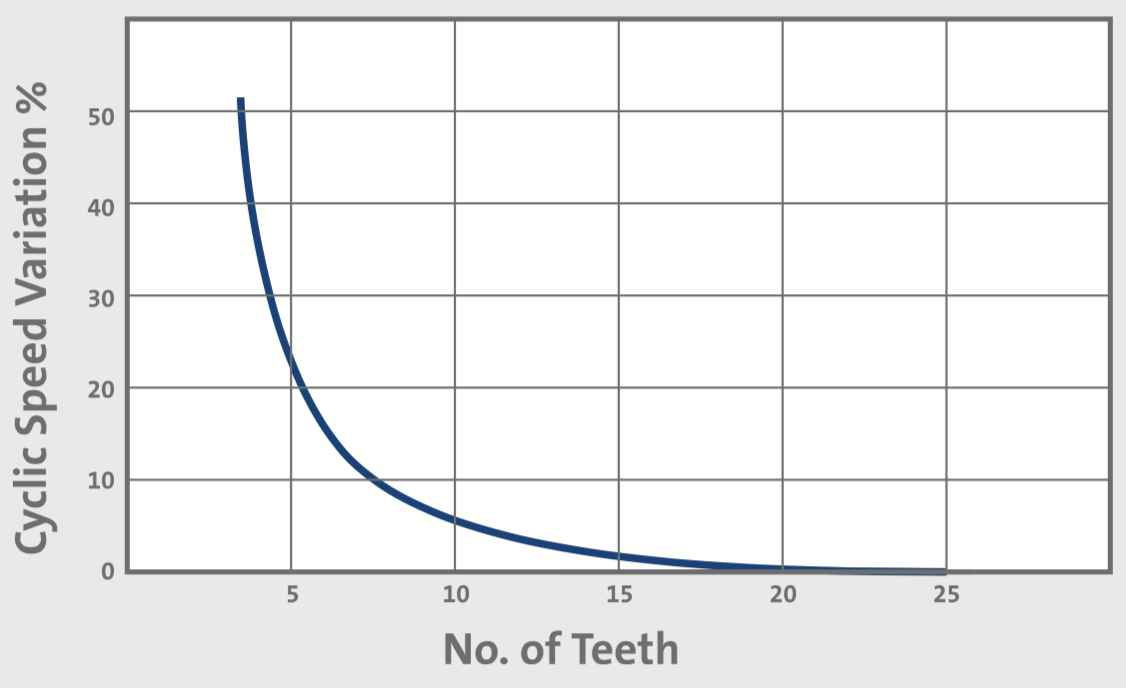
\includegraphics[width=\textwidth]{figs/polygonal-action.png}
  \caption[Cyclic speed variation due to polygonal action]{Cyclic speed variation due to polygonal action~\citep[p.24]{renoldchain}}
  \label{fig-cyclic-speed-variation}
\end{marginfigure}

It\marginnote{cranked link} is always best practice and desirable to have a chain with an even number of links. However, when there is a case that requires an odd linked chain, cranked links are used to form the chain loop. \cref{fig-cranked-link} shows an example of a cranked link within a chain. The link has a natural kink in the profile to allow it to connect to the next link in the chain. This inherently places additional stress concentrations within the component and thus, is not recommended for high load and/or speed chain drives.


\begin{marginfigure}
  \centering
  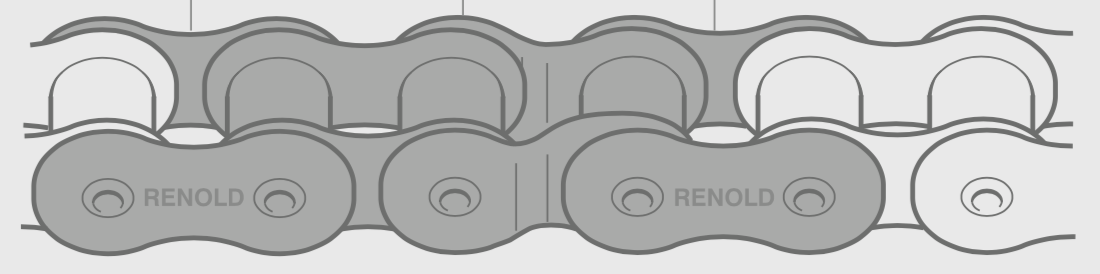
\includegraphics[width=\textwidth]{figs/cranked-link.png}
  \caption[Cranked link]{Cranked link~\citep[p.11]{renoldchain}}
  \label{fig-cranked-link}
\end{marginfigure}

\subsubsection{Selection Process}

The selection process for a Renold chain is as follows. The prerequisites for the process is that you know the torque and sprocket speeds that you wish to run at.

%\begin{enumerate}
%  \item Calculate your requirements
%  \begin{itemize}
%    \item Transmission ratio
%    \item Speeds of the driving and driven sprockets
%    \item Torque transmitted
%    \item Power
%    \item Force in the chain
%  \end{itemize}
%  \item Find a suitable chain pitch, select chain and sprockets
%  \item Calculate the chain length and centre distance
%\end{enumerate}

The\marginnote{Selection Power (\(P_s\))} selection power is calculated by multiplying the power you wish to transmit (\(P_s\)) by two safety factors \(f_1\) and \(f_2\).

\begin{equation}
  P_s = f_1f_2P_t
\end{equation}

\noindent Where:

\begin{description}
  \item[\(f_1\)] Safety factor depending on your operation and can be found using chart 2 on p.28 of the Renold catalogue
  \item[\(f_2\)] Adjustment factor is your are using the non-recommended number of driving sprocket teeth. \(f_2=\frac{19}{\text{No. of teeth on driving}}\)
\end{description}

With\marginnote{Selecting a Suitable Chain Pitch} the selection power determined and the driver sprocket speed known, one can determine the chain pitch using \cref{fig-chain-pitch}. These rating charts have been created from years of empirical testing and theoretical modelling by the chain companies, and dictate the safe operating windows for their selection of chains.

\begin{figure}[h!]
  \centering
  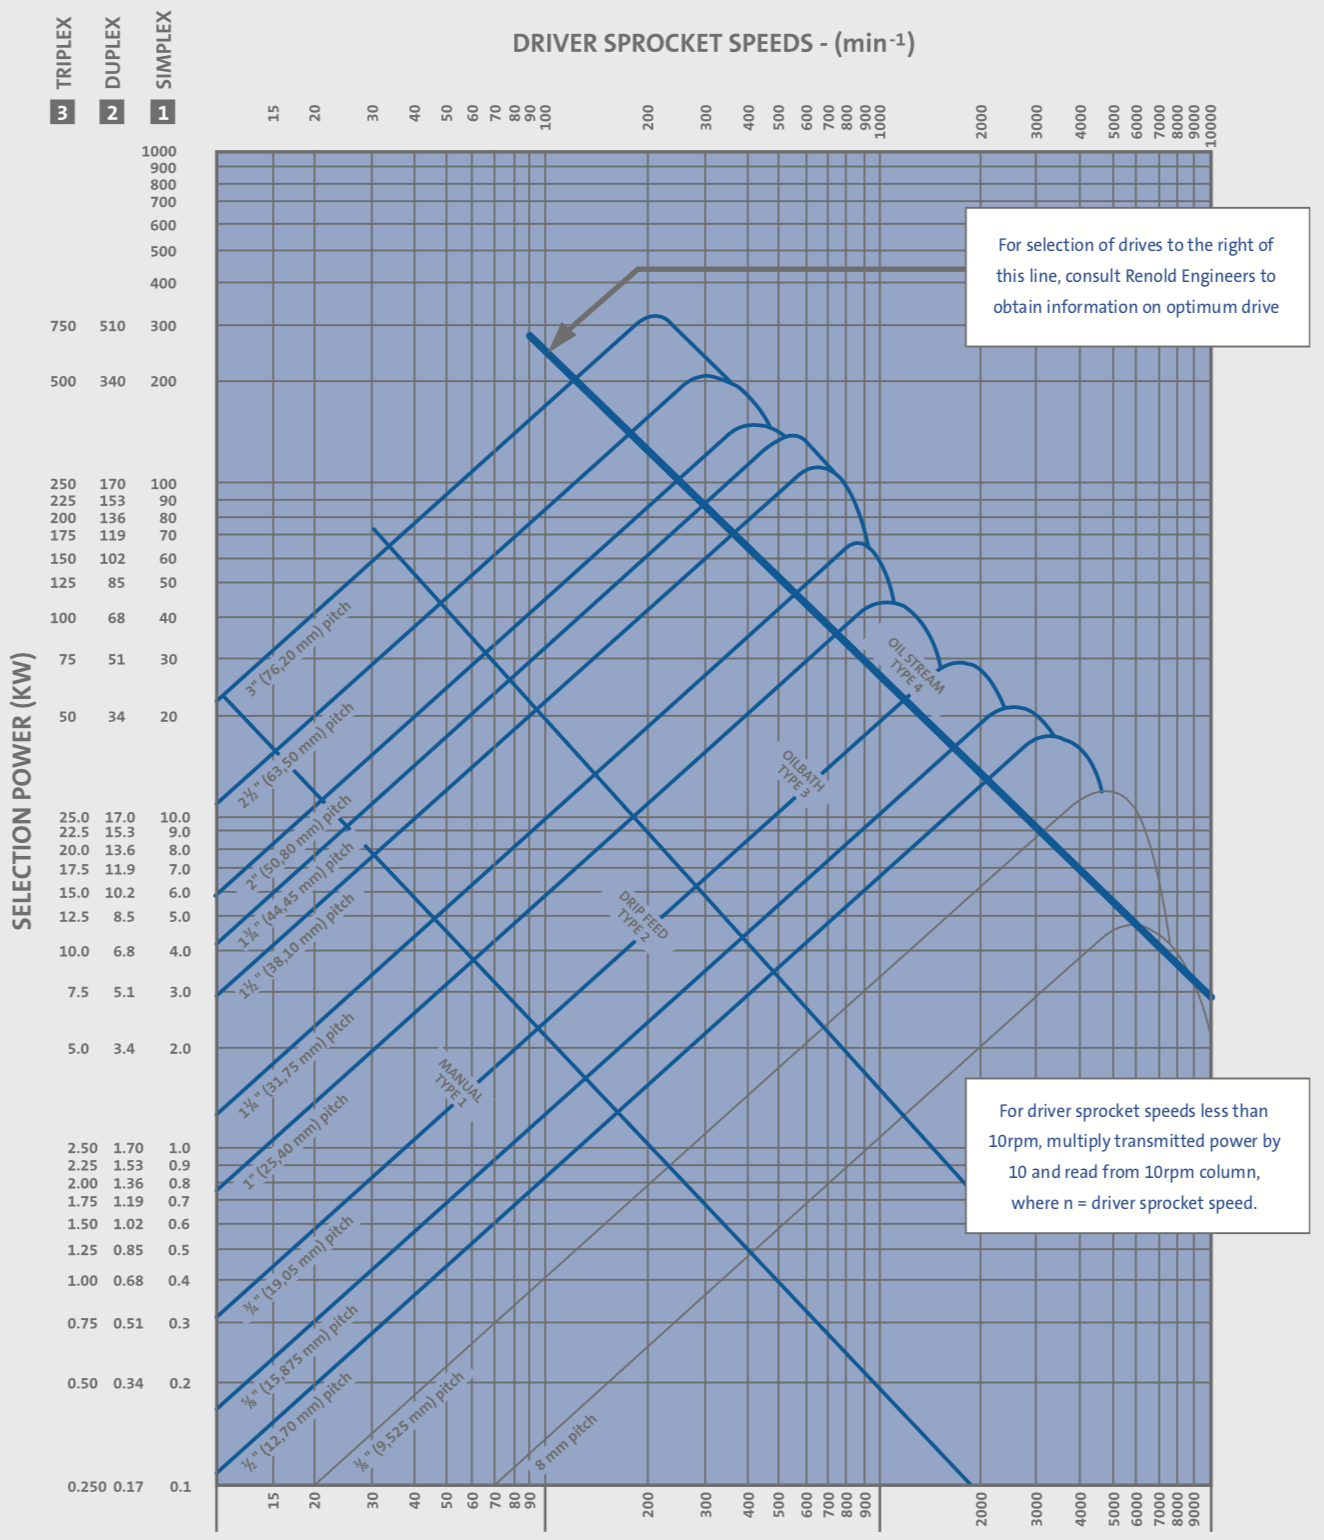
\includegraphics[width=0.9\textwidth]{figs/chain-pitch.png}
  \caption[Chain pitch selection chart]{Chain pitch selection chart~\citep[p.31]{renoldchain}}
  \label{fig-chain-pitch}
\end{figure}

After\marginnote{Select Chain and Sprockets} selecting the chain pitch, you can go through the catalogue to find the drive and driven sprockets that will give you the required (or as near as possible) ratio for your design.

Having\marginnote{Chain Links and Centre Distance} the chain pitch and sprockets selected, the centre distance

\begin{equation}
  L = \frac{Z_1+Z_2}{2}+\frac{2C_1}{P}+\frac{P{\left(\frac{Z_2-Z_1}{2\pi}\right)}^2}{C_1}
\end{equation}

\noindent{} Where:

\begin{description}
  \item[\(Z_1\)] Number of driving teeth
  \item[\(Z_2\)] Number of driven teeth
  \item[\(C_1\)] Approximate desired centre distance
  \item[\(P\)] Chain pitch
  \item[\(L\)] Number of chain links
\end{description}

Once calculated, you then round to the nearest even integer and use this to calculate your centre distance \(C\).

\begin{equation}
  C=\frac{P}{8}
  \left[
  2L-Z_2-Z_1 
  +
  \sqrt{ 
    {\left(2L-Z_2-z_1\right)}^2 - \left(\frac{\pi}{3.88}\left(Z_2-Z_1\right)^2\right)
  }
  \right]
\end{equation}

\subsubsection{Chain Example}

Select a chain and sprocket to transmit \SI{2}{\kilo\watt} of power at \SI{20}{rpm}. A ratio of 1:2 is required, driven by an electric motor with moderate shocks expected from the load. Space is highly limited.

Using\marginnote{determining \(f_1\) and \(f_2\)} Chart 2 on p.28 of the Renold catalogue, we identify that \(f_1=1.4\) for our context and we will also use the recommended number of teeth on the driving sprocket (19), which makes \(f_2=1\). Therfore, the selection power \(P_s\) becomes:

\begin{equation}
  P_s = f_1f_2P_t = 2\si{\kilo\watt}\times1.4\times1=2.8\si{\kilo\watt}
\end{equation}

Using\marginnote{chain pitch} \cref{fig-chain-pitch}, we can find the chain pitches that are suitable for our application. The potential pitches are:

\begin{itemize}
  \item \SI{38.10}{\milli\metre} simplex
  \item \SI{31.75}{\milli\metre} duplex
  \item \SI{25.40}{\milli\metre} triplex
\end{itemize}

For\marginnote{chain and sprocket selection} this example, we will select the triplex as our requirement is to have a compact solution. Now it is just a case of looking in the tables to find a sprocket set (Renolds, p.75) that will provide us with a ratio that provides us with the closest match in terms of our desired ratio, and a triplex chain (Renolds, p.25).

\begin{description}
  \item[Chain] 12B-3
  \item[Driving Sprocket] 16B1/19T
  \item[Driven Sprocket] 16B1/38T
\end{description}

Now\marginnote{chain links} we have the sprockets and chain selected, it is then a simple case of using their specifications to determine the number of links:

\begin{equation}
  L = 
  \frac{19+38}{2}
  +
  \frac{2\times571.5}{19.05}+\frac{19.05{\left(\frac{38-19}{2\pi}\right)}^2}{571.5} = 88.6
\end{equation}

Rounding this up to the nearest even integer gives us \(L=90\).

The\marginnote{centre distance} final calculation is to determine the centre distance:

% https://www.sharelatex.com/learn/Aligning_equations_with_amsmath
\begin{equation}
\begin{split}
  C & = \frac{19.05}{8}
  \left[
  2(90)-38-19 
  +
  \sqrt{ 
    {\left(2(90)-38-19\right)}^2 - \left(\frac{\pi}{3.88}\left(38-19\right)^2\right)
  }
  \right] 
  \\ & = \SI{583}{\milli\metre}
\end{split}
\end{equation}

\subsection{Selecting a vee-belt or tooth belt}

\begin{framed}
  \vspace{1cm}
    \begin{center}
      {\fontsize{50}{60}\selectfont ?}\\
      Own Research \& Lectures
    \end{center}
  \vspace{1cm}
\end{framed}

%\subsection{Selecting a tooth belt}

%\begin{framed}
%  \vspace{2cm}
%    \begin{center}
%      {\fontsize{50}{60}\selectfont \faQuestion{}}\\
%      Research Required
%    \end{center}
%  \vspace{2cm}
%\end{framed}
